
\documentclass[conference,compsoc]{IEEEtran}
\ifCLASSOPTIONcompsoc
  \usepackage[nocompress]{cite}
\else
  \usepackage{cite}
\fi
\ifCLASSINFOpdf
   \usepackage[pdftex]{graphicx}
\else
\fi
\hyphenation{op-tical net-works semi-conduc-tor}


\begin{document}
\title{Exploratory Analysis of various algorithms on Student Performance Data using Machine Learning}
\author{\IEEEauthorblockN{Shubham Barudwale\IEEEauthorrefmark{1},
\IEEEauthorblockA{\IEEEauthorrefmark{1}School of Computing Sciences and Engineering, 
VIT Chennai, Tamilnadu, India 600127\\
Email: barudwaleshubham.dinesh2015@vit.ac.in\IEEEauthorrefmark{1}}
}
}
\maketitle

\begin{abstract}
	Academics is the major part of the life across all the fields. While persuing any course the understanding is measured using the marks in the exam generally across the world. The academic performance can be affected by various factors like family, society, lifestyle and so on. So the motive of this study is to find out what are the factors that plays major roles in the academic performance and how we can learn the facts and predict the academic performance using machine learning. Also the paper will discuss the algorithms used and in what conditions the algorithms will work efficiently.
	

	In this study the data has been analysed and tried to be learn the underlying information using many experiments. This paper explains the comparetive study between all the algorithms that had been performed on the data and tells the results observed. The maximum accuracy achieved was 96.41\%
\end{abstract}
\section{Keywords}
	Machine Learning, Comparitive analysis, Student Data 



\section{Introduction}
The main problem to be solved is analyse the data and to predict the results for given cases. The data had been trained using different algorithms in Machine learning. 

There the analysis is used using both superwised and unsuperwised learning methods.
In supervised methods the algorithm uses the predefined correct output of the data for training the model. On other hand unsuperwised learning only takes the data and try to find the useful meaning out of it. In the experiments performed in this paper the each algorithm and methods are useful for some specific types of data. 

Some algorithms are useful whare the classification of two classes has to be made. e.g. class A and B. In some cases the data given is in clustered form. The data given can be descrete, continuous or mixture of both. So for each dataset the methods to be used can differ. So to understand the algorithms well discussion of aspects, results, pros-cons and the usability of algorithms will be disscussed in the upcoming topics. 


\section{Database - Iris dataset}
Student performance dataset is the dataset from which we are trying to gain some information from 650 student’s academic performance data and various attributes which are affecting the performance. Attributes include sex, age, study time, free time, family information etc.
 
We will be using various algorithms listed below to learn and predict the performance. Out of 650 I have taken 455 data entries for lerning and rest for prediction i.e testing performance of the algorithm.(70:30). The labels or target functions are mentioned in the ‘new’ field which is added manually. bad(0-7), medium(8-14), good(15-20).
 

\section{Algorithms}
1. Data Preprocessing

2. Perceptron Algorithm

3. Decision Trees

4. Logistic Regression

5. Regression

6. K-means Clustring

7. Neural Networks

8. Support Vector Machine

9. K Nearest Neighbours



\section{Methodology}

The data given was in the form of string input which was converted to the numeric descrete data. Then the data was analysed using various Exloratory Data Analysis Techniques(EDA). Some outliers were found in the process which were retained or discarded according to the algorithm applied to learn dataset. The data was divided into 70:30 train test parts to check accuracy of the given algorithm on test data. Then training was done on the data and test data was tested for each algorithm seperately to get the accuracy. The performance improvement was done using methods like pruning, dimentionality reduction, changing the paremeters on which the data was trained.\\

Noisy data can contain duplicate data,
improper data, missing values, text data. To
make data clean we can either ignore the dirty
data or can assign some values based on other
values of the same field. While preprocessin the
data we will check for duplicate entries and we
will delete them. For missing data we can ignore
them or assign the zero values. The better
method to deal with such data is to take average
of the data in the same field and put the value in
the missing places so that the generalization can
done. We cannot deal with text while drawing
the decision boundries so to reinforce that we
use the temporary aasignment values for each
unique text field.By plotting the scatter graphs, seeing the
mean and mode plots and values we can easily
identify the outliers in the data. Graphical
methods are very useful in such data
preprocessing techniques. Here as the data was in the string format the data cleaning was done
and the data was converted into the numeric data.\\

As perceptron is basic algorithm used for the primary classification the data
was trained using perceptron. The perceptron algorithm is used in
neural networks. A perceptron is an artificial
neuron which works on threshold logic. It
accepts multiple inputs e.g. ${x1,x2,x3,....xn}$ with
weights which are summed up. If sum is greater
than the threshold then the neuron gets asserted
and the point is labeled as one class, if neuron
does not get asserted then the datapoint belongs
to another class. Inputs and weights are
generally real values, weights are the
importance of the filed in the given dataset
which can be negative.
According to threshold the algorithm
will be dividing the data into two classes which
are seperated by either line for 2D or plane for
3D or hyperplance in higher dimensions. The
perceptron is majorly used to classify the
linearly sepearble data. The perceptron algorithm is good if the data is linearly seperable. If the data is not linearly seprable then the perceptron does not work well. Perceptron algorithm is a primitive algorithm to classify the data bases on supervised learning. Here data was not exactly liniarly seperable in 2 and three class so the accuracy was low so the decision was to apply another algorithms.\\

The data given was the descrete data so the decision trees was the better option.
Decision trees work better in distinguishing the points based on different characters 
which are different from each other distinctively. 
Decision trees are non parametric
supervised learning method used for
classification and regression. Decision tree
creates the model to predict the decision by
creating simple decision rules.
Decision tree takes attributes of the data
and try to figure out the importance of each data
field according to the target function. It classifies (or splits) the whole data based on
such decision making trees. We can give the
depth of the tree upto which the algorithm will
consider various attributes of the data and will
classify them upto n depth. More the depth
means more will be the accuracy based on
various attributes.
Some of advantages of the decision trees
are, they are simple to understand and to
interrupt. They can be visualized. Time required
to train and prediction reduces exponentially.
Able to handle any type of data. Validation is
easy using statistics.
But in some cases where data is not
simple overfitting can happen by complex trees.
Small variation in data can give completely
different tree. Could crete biased trees if some
classes are dominant. This time the model gave better results. \\

Probability of a point to belong to a particular class can be seen as useful resource
We can calculate the future probabilities based on the values we get. 
In logistic regression we need to restrict
the hard threshold of linear classification
because linear regression does not use threshold.

After confining the output values we
find the probabilistic value of the function using
conditional probability. Which gives us the
probability of a point belonging to one class.

After this also there can be misclassified
points which will increase the probability of
having the wrong group then we will apply most
likelihood methods and gradient descent to
inprove the corret probability by taking the
smaller steps.
Linear classification uses a hard
threshold on the signal 

In Logistic regression, we need something in
between these two cases that smoothly
restricts the output to the probability range
$[O, l]$.
One choice that accomplishes this goal is
the logistic regression model
 whose output is between 0 and 1
 
We are trying to learn the target function
The data does not give us the value off
explicitly. Rather, it gives us samples
generated by this probability. Therefore, the data
is in fact generated by a noisy target
The standard error measure $e(h(x), y)$ used in
logistic regression is based on the notion of
likelihood; how 'likely' is it that we would get
this output $y$ from the input $x$ if the target
distribution $P(y I x)$ was indeed
captured by our hypothesis $h(x)$.The main advantage of the logistic regression is the regression gives the probability of group to which the point belongs.\\

Until now superwised models were trained on the data and we got medium to good results
testing the data without knowing the output could give some insights of the data.
Unsuperwised learning is the learning
from the data where the target value is not
given. Linear regression is also a algorithm
which uses the unsuperwised learning method to
fit and learn some knowledge out of the given
data.
In linear regression we try to fit the data
with a stright line which reduces the mean
sqquare errors between the points and line.
To minimize the calculations we use the pseudoinverse method. In which the X is matrix of
attribute values and y is our hypothesis line.
We also used the RANSAC algorithm
which reduces the effect of outliers on fitting.

The linear regression algorithm is based
on minimizing the squared error between $h(x)$
and $y.2$
$Eout(h) = E [(h(x)- y)^2]$
where the expected value is taken with respect
to the joint probability distribution $P(x, y)$. The
goal is to find a hypothesis that achieves a small
$Eout(h)$.The main advantage is that the regression can learn the continuous data even if the output is unknown but this fails if the data given is descrete or in the forms of cluster.
But as the data in our dataset was not continuous the regression model could not give good results.\\

I have also tried to cluster the data into number of clusters using various methods like K means, K modes, KNN etc.
K-Means is the algorithm in which the
data is divided into K clusters. First the K
centreroids are defined randomly. In case of K
Means++ it centeroids are taken as far as
possible. Then each points are assigned to the
nearest centeroids. And again the centeroid is
calculated of those clustered data. Then again
several times the procedure is repeated until no
points are altered.
This method is very useful for the
distinctive data which can be visualized as
groups.

We can define similarity as the opposite of
distance, and a commonly used distance for
clustering samples with continuous features is
the squared Euclidean distance between two
points x and y in m-dimensional space

$d(x,y)^2 = \sum(x_{j}-y_{j})^2 = ||x-y||^2$\\
Note that, in the preceding equation, the index j
refers to the jth dimension (feature column) of
the sample points x and y. In the rest of this
section, we will use the superscripts i and j to
refer to the sample index and cluster index,
respectively. Based on this Euclidean distance
metric, we can describe the k-means algorithm
as a simple optimization problem, an iterative
approach for minimizing the withincluster sum
of squared errors (SSE), which is sometimes
also called cluster inertia.
The algorithm is useful when the distinguishing clusters are present in the data and the target function is unknown or the output and the class o the data is unknown. But as each time the distance between all points has to be found the compuationally k-means is costly. \\

After training data on all the above models we found that the data is not linearly seperable, nor clustered. Also the data was not continuous so regression also failed. So the option to get the appropriate good results was to see all the data points one by one and learn them by adjusting the logic based on output ao here we opted for Neural Networks.
Artificial neural networks (ANNs) or
connectionist systems are computing systems
inspired by the biological neural networks that
constitute animal brains. Such systems learn
(progressively improve performance) to do tasks
by considering examples, generally without
task-specific programming.

An ANN is based on a collection of
connected units called artificial neurons,
(analogous to axons in a biological brain). Each
connection (synapse) between neurons can
transmit a signal to another neuron. The
receiving (postsynaptic) neuron can process the
signal(s) and then signal downstream neurons
connected to it. Neurons may have state, and
weight generally represented by real numbers,
typically between 0 and 1. Using states and
weights and adjusting them the ANN decides
the final output.

In Multilayer Neural Networks generally
used algoritm is backpropogation method. In
this method first the values are feeded into the
first layer of the network. And the next several
layers are connected by the weigths. The values
of the next layer’s nodes are calculated by
multiplying the input values and weights. And
the same method is applied until the terminal
output layer is reached.
Then if the output values are not distinct
and close to the required values then again the
values are backpropogated in oredr to change
the weigts of the links and again the values are
calculated for several times. The activation method used are sigmoid, tanh etc.

The speciality of neural netwoks is it can learn and adjust itself bases on the previous all the data points trained on it. The hidden featurs also can be learned using the neural network. Complex data sets like XOR can be solved using only 1 hidden layer. The application of the neural network is vast in the case where distinct features cannot be extracted easily.\\

For more experiments the following models were also trained. But the results obtained were not giving good accuracy.
Support Vector Machine (SVM) is the
superwised learning algorithm. In perceptron we
have seen that the differentiation line/ classifier
line can be any line between the two groups. It
can cause some errors in the test data by
classifying the data incorrectly. That is
generalization of the data can be not correct
always.
To overcome this the SVM is the best for
getting the clear and optimal classification line.
Which is equidistant from both the classes and
can classify the data optimally.
The given images shows that how
perceptron works in classification and how
SVM gives better results on the same data with
maximum margin to accomodate the test data.

SVM can be used in the conditions
where the training points are less than 1000
because the only poits matters to draw the SVM
classifier line is the Support vectors. In SVM
the main goal of the algorithm is to maximize
the margin between the points and the classifier
line. When the data is not linearly seperable
the the transformation takes place and the data is
transferred to the higher dimensions and then it
is classified. The method uses the various
transform functions. Which is called the Kernal
trick\\

K Nearest Neighbour (KNN) algorithm
is the algorithm in which the classification of
the test data is done by using its neighbour’s
properties and calss. In KNN the training part is
not consided that is why its only the observe and
classify the data.

In KNN algorithm following steps takes
place:

1. Choose the number of k and a distance
metric.

2. Find the k nearest neighbors of the sample
that we want to classify.

3. Assign the class label by majority vote.

K in the KNN is always odd. So that the
both class numbers are not even.
The point to be classified finds the
distance between all the points in the cluster and
takes K nearest neighbours and finds the most
number of the classes in the k neighbours and
point belongs to the class which are more in
numbers in k.

Once the data point is classified then that
point is also included into the pool of the points
to classify the further points. This is called the
memory based approch. The main advantage of
such a memory-based approach is that the
classifier immediately adapts as we collect new
training data. However, the downside is that
the computational complexity for classifying
new samples grows linearly with the number of
samples in the training dataset in the worst-case
scenario—unless the dataset has very few
dimensions (features) and the algorithm has
been implemented using efficient data structures
such as KD-trees.
The distance is calculated by many
distance formulas. But the most used formula is
Euclidian distance

Some of the varients of the KNN uses the
weighted distances by giving more weights to
some of the attributes. So that the classification
takes place correctly.
When we consider the data in the higher
dimensions the nearest points might be far away
from the point to be classified.\\





\section{Experiments}
First data preprocessing was performed on the data to convert the data from string data to numeric data. Then the data was tested using various statistical methods. From the mean of the all feilds the data was majorly talking about the school students in the grade 9th , 10th and the average marks were 11/20. The Study time was increased as the marks were more. As the data was descrete the data was not interpreted from the pairplot and other graphs properly. 

The perceptron is the basic superwised algorithm which divides the data into classes by trying to adjust weights and try to make a straight line to divide the data. After 100 iterations the misclassifications were dropped to 5. The accuracy obtained by the perceptron was 88.2\%.

In Decision trees the features are extrcted according to the significant division. And the tree is created upto the depth 3.  The accuracy on test data was 94.4\%. 
\begin{figure}
	\centering
		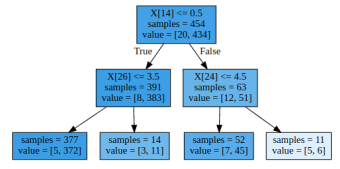
\includegraphics[width=3.5in,height=1.8in]{DT_IMG.png}
	\caption{Decision Tree}
	\label{fig_1}
	
\end{figure}

\begin{figure}
	\centering
	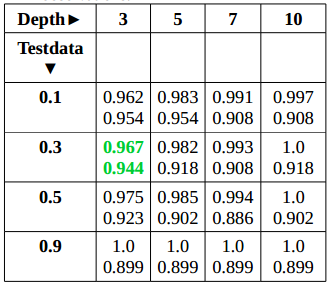
\includegraphics[width=3.5in,height=1.8in]{DT.png}
	\caption{Decision Tree Results}
	\label{fig_2}
\end{figure}

The Logistic regression predicts the probability of each data point to be a part of a group. The accuracy of the data was not good since the probabilitis were very close to each other and the data in this case was not very well differentiable. So the Logistic regression could not give the proper results of the regression on student performance data.

In simple regression as the data is discrete the regression did’t work as expected. Some graphs could make the sence but the most of them were redundant according to the observation.


 The next algorithm used was clustring algorithm which was unsuperwised learning algorithm. In which the clusters are made by taking the minimum distance from points and clustering them together. As we made three clusters the descrete data could not make correct clusters and the clusters were incorrect.
 
 The neural network was the one which gave the highest accuracy in the testing among the all algorithms used wchich was 96.41\%. So as the backpropogation method is used in the neural networks the weights of the edges in the neural network will adjust with itself to give accuate results. These results were very good compared to other advaced models like XGBoost where multiple models are mixed to give better results.The computation required in this model is also less and only gives fifference about 3\% accuracy. So overall the neural network is tradeoff between computation and results.
 
 \begin{figure}
 	\centering
 	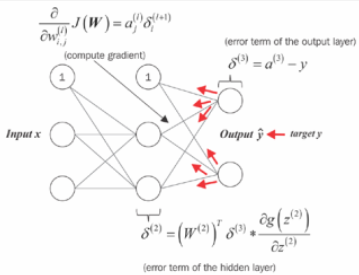
\includegraphics[width=3.5in,height=1.8in]{NEURAL.png}
 	\caption{Neural Networks}
 	\label{fig_3}
 \end{figure}

 Support Vector Machine the advanced version of the perceptron in wchich we try to find the maximum margin classifier to classify the points into different classes. As the data is overlapped the SVM could not find the good classifier in 2 dimension representation. Same results were observed in the KNN algorithm as the classes are not well distinguihable the clusters formed by selecting K nearest points and assigning the class that the maximum neighours belong to were not promisable. The accuracy observed was 74.35\%
 

 
 Here from the various experiments we can see that the regression and clustering algorithm didn’t perform well as the data was discerete. The Decision tree performed better since the significant attributes were anaysed and the tree was created to classify the data. The best results obtained was using neural networks since the tree adjusts the weights using the previous all the records in training and uses it for the prediction.
 


\section{Conclusion}

Descrete data is learned by algorithms like Decision Trees and Neural Networks well. The Student Data could not be learned by the regression and clustering since the data was descrete. The accuracy of the Decision Trees was 94.4\% and the Neural Network was 96.41\% Neural netowrk works best for the data which is descrete and which cannot be leaned through regular methods. Neural network is the tradeoff between highly compound models like XGBoost which takes high computation and accuracy by using simple model.


\section{Referances}

1)	http://scikit-learn.org

2)	https://www.kaggle.com

3)	Python Machine Learning, $Sebastian Raschka$

4)	Learning From Data, $Yaser S. Abu Mostafa$

5)	DATA CLUSTERING, $Charu C. Aggarwal$

\ifCLASSOPTIONcompsoc
\fi



\bibliographystyle{IEEEtran}
\bibliography{Final.bib}


\end{document}



